\documentclass[11pt,a4paper]{article}

\usepackage[utf8]{inputenc}
\usepackage[T1]{fontenc}
\usepackage[spanish,es-tabla]{babel}
\usepackage{csquotes}
\usepackage[margin=2.5cm]{geometry}
\usepackage{graphicx}
\usepackage{booktabs}
\usepackage[hidelinks]{hyperref}

\usepackage[
  backend=biber,
  style=ieee,
  sorting=none
]{biblatex}
\addbibresource{referencias.bib}

\graphicspath{{img/}}

\begin{document}

% ------------------------------------------------------------------------------
% Caratula institucional
% ------------------------------------------------------------------------------
\begin{titlepage}
  \centering
  \vspace*{0.8cm}

  {\Large \textbf{UNIVERSIDAD T\'ECNICA ESTATAL DE QUEVEDO}\par}
  \vspace{0.3cm}
  {\large Facultad de Ciencias de la Computaci\'on\par}
  {\large Carrera de Software\par}

  \vspace{1.4cm}
  {\LARGE \textbf{FORM-IC-01 --- Investigaci\'on Individual}\par}
  \vspace{0.3cm}
  {\Large \textbf{Arquitecturas Distribuidas en la Industria}\par}
  \vspace{0.6cm}
  {\large Caso de estudio: Datalex \textbar{} Patr\'on arquitect\'onico: API Gateway\par}

  \vspace{1.4cm}
  \begin{tabular}{ll}
    \textbf{Asignatura:}                & Aplicaciones Distribuidas \\
    \textbf{C\'odigo:}                  & ISR-701 \\
    \textbf{Docente:}                   & Gleiston Cicer\'on Guerrero Ulloa, PhD \\
    \textbf{Estudiante:}                & Luis Alberto Paca Pilataza \\
    \textbf{Nivel:}                     & S\'eptimo \\
    \textbf{Paralelo:}                  & A \\
    \textbf{Per\'iodo acad\'emico:}     & SPA 2026--2027 \\
    \textbf{Semana:}                    & 5 \\
    \textbf{Modalidad:}                 & Individual \\
    \textbf{Actividad:}                 & FORM-IC-01 --- Investigaci\'on Individual \\
    \textbf{Caso de estudio:}           & Datalex \\
    \textbf{Patr\'on arquitect\'onico:} & API Gateway \\
    \textbf{Fecha:}                     & 28 de noviembre de 2026 \\
  \end{tabular}

  \vfill
  {\small Documento en preparaci\'on: contenido anal\'itico pendiente de redacci\'on propia del estudiante.\par}
\end{titlepage}

% ------------------------------------------------------------------------------
% Analisis del caso Datalex (extension objetivo: UNA SOLA pagina)
% ------------------------------------------------------------------------------
\section*{An\'alisis del caso Datalex}

\subsection*{A. Descripci\'on del caso}
Datalex es una empresa especializada en soluciones de comercio electr\'onico para aerol\'ineas, orientadas a la gesti\'on de precios, b\'usquedas comerciales y pedidos. El caso analizado corresponde a la migraci\'on de su capa de integraci\'on mediante API REST hacia Amazon API Gateway, abarcando entornos de producci\'on y no producci\'on en aproximadamente dos semanas~\cite{prenty2020datalex}. La compatibilidad de los contratos de API fue un requisito cr\'itico para preservar la interoperabilidad con aplicaciones externas y evitar interrupciones en sus procesos de negocio~\cite{prenty2020datalex}. La fuente~\cite{prenty2020datalex} no especifica el volumen de solicitudes ni la cantidad de usuarios.

\subsection*{B. Elecci\'on del patr\'on arquitect\'onico}
La soluci\'on anterior presentaba limitaciones t\'ecnicas y econ\'omicas asociadas a contratos multianuales con pagos fijos, creaci\'on manual de API y ausencia de cuotas individuales~\cite{prenty2020datalex}. Amazon API Gateway permiti\'o adoptar un modelo de pago por consumo, compatibilidad con OpenAPI y gesti\'on granular del tr\'afico mediante planes de uso y mecanismos de \textit{throttling}~\cite{prenty2020datalex}. Estas capacidades justifican la elecci\'on desde una perspectiva de eficiencia operativa~\cite{aydemir2025apigateway,moreira2023age}. No obstante, se identifica como compromiso arquitect\'onico la dependencia tecnol\'ogica (\textit{vendor lock-in}) del ecosistema AWS, que podr\'ia incrementar la complejidad y los costos de una futura migraci\'on.

\subsection*{C. Beneficios obtenidos}
\textit{[Pendiente de redacci\'on propia del estudiante: beneficios operativos y resultados medibles verificados (alcance exacto del ahorro de casi el 98 \%, plazo de dos semanas y continuidad reportada), diferenciando evidencia empresarial de limitaciones de medici\'on. Referencias previstas: \texttt{\textbackslash cite\{prenty2020datalex\}}, \texttt{\textbackslash cite\{aydemir2025apigateway\}}, \texttt{\textbackslash cite\{moreira2023age\}}.]}

\subsection*{D. Desaf\'ios y soluciones}
\textit{[Pendiente de redacci\'on propia del estudiante: retos t\'ecnicos de compatibilidad hacia atr\'as y continuidad, soluci\'on en dos fases (Lambda Custom Authorizer con \texttt{usageIdentifierKey} y corte CNAME; CloudFormation y cabecera nativa \texttt{x-api-key}) y compromisos arquitect\'onicos o \textit{trade-offs}. Referencias previstas: \texttt{\textbackslash cite\{prenty2020datalex\}}, \texttt{\textbackslash cite\{moreira2023age\}}.]}

\subsection*{E. Aplicaci\'on al Proyecto Fin de Curso}
\textit{[Pendiente de confirmaci\'on del PFC de Aplicaciones Distribuidas y redacci\'on propia del estudiante: qu\'e pr\'acticas de Datalex adoptar y cu\'ales descartar seg\'un escala, complejidad operativa, costos y dependencia tecnol\'ogica. Referencias previstas: \texttt{\textbackslash cite\{prenty2020datalex\}}, \texttt{\textbackslash cite\{aydemir2025apigateway\}}, \texttt{\textbackslash cite\{moreira2023age\}}.]}

\clearpage

% ------------------------------------------------------------------------------
% Evidencias de autoria (seccion diferenciada del analisis de una pagina)
% ------------------------------------------------------------------------------
\section*{Evidencias de autor\'ia}

\subsection*{Evidencia de lectura de la fuente principal}
Las Figuras~\ref{fig:evidencia_01} a~\ref{fig:evidencia_04} recogen las capturas reales de la lectura y el subrayado personal realizados por el estudiante sobre la publicaci\'on oficial de AWS acerca del caso Datalex~\cite{prenty2020datalex}.

\begin{figure}[htbp]
  \centering
  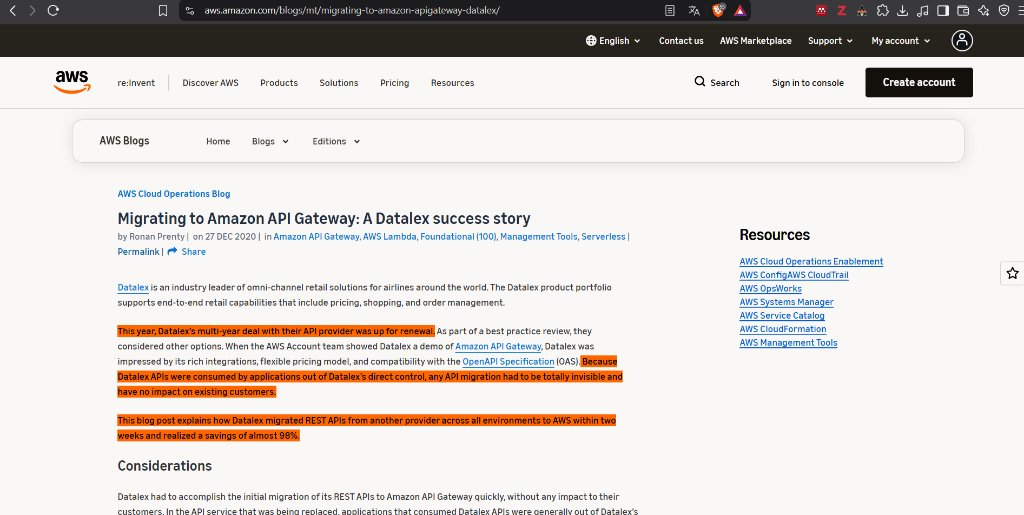
\includegraphics[width=0.92\linewidth]{evidencia_01_intro_considerations.jpg}
  \caption{Evidencia de lectura y subrayado personal del apartado introductorio de la fuente oficial: renovaci\'on contractual, restricci\'on de migraci\'on invisible, plazo de dos semanas y ahorro reportado de casi el 98 \%. Fuente: Prenty, Morrow y Galan~\cite{prenty2020datalex}.}
  \label{fig:evidencia_01}
\end{figure}

\begin{figure}[htbp]
  \centering
  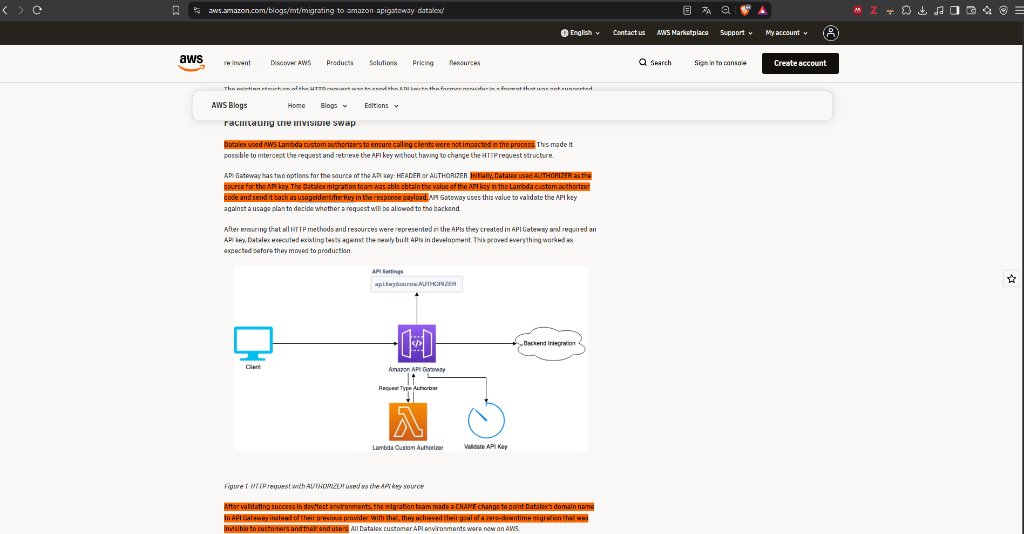
\includegraphics[width=0.92\linewidth]{evidencia_02_fase1_lambda_cname.jpg}
  \caption{Evidencia de lectura y subrayado personal de la primera fase (\textit{Facilitating the invisible swap}): uso de \texttt{apiKeySource: AUTHORIZER}, autorizador personalizado en AWS Lambda (\texttt{usageIdentifierKey}), Figura~1 original y cambio DNS mediante registro CNAME. Fuente: Prenty, Morrow y Galan~\cite{prenty2020datalex}.}
  \label{fig:evidencia_02}
\end{figure}

\begin{figure}[htbp]
  \centering
  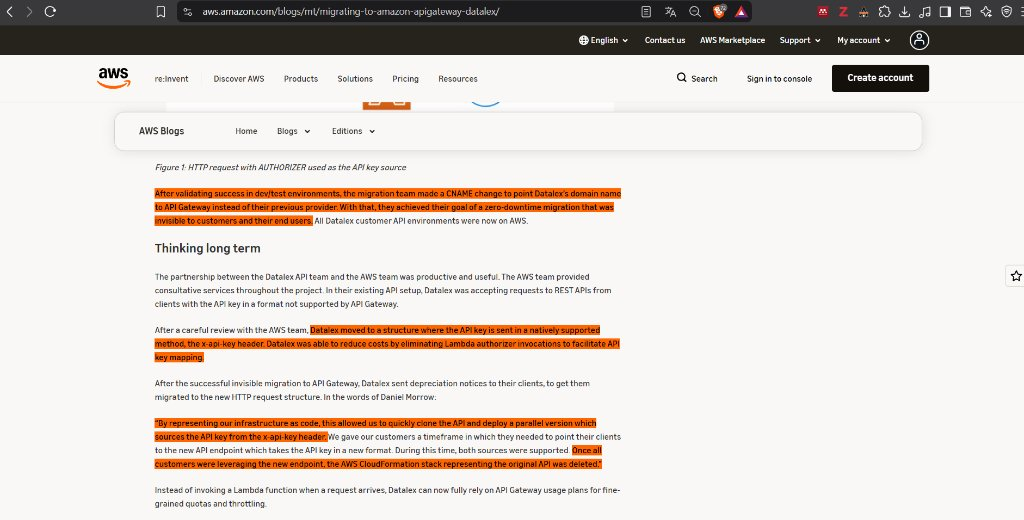
\includegraphics[width=0.92\linewidth]{evidencia_03_fase2_cloudformation.jpg}
  \caption{Evidencia de lectura y subrayado personal de la segunda fase (\textit{Thinking long term}): transici\'on hacia la cabecera nativa \texttt{x-api-key}, clonaci\'on paralela mediante AWS CloudFormation y eliminaci\'on del \textit{stack} original. Fuente: Prenty, Morrow y Galan~\cite{prenty2020datalex}.}
  \label{fig:evidencia_03}
\end{figure}

\begin{figure}[htbp]
  \centering
  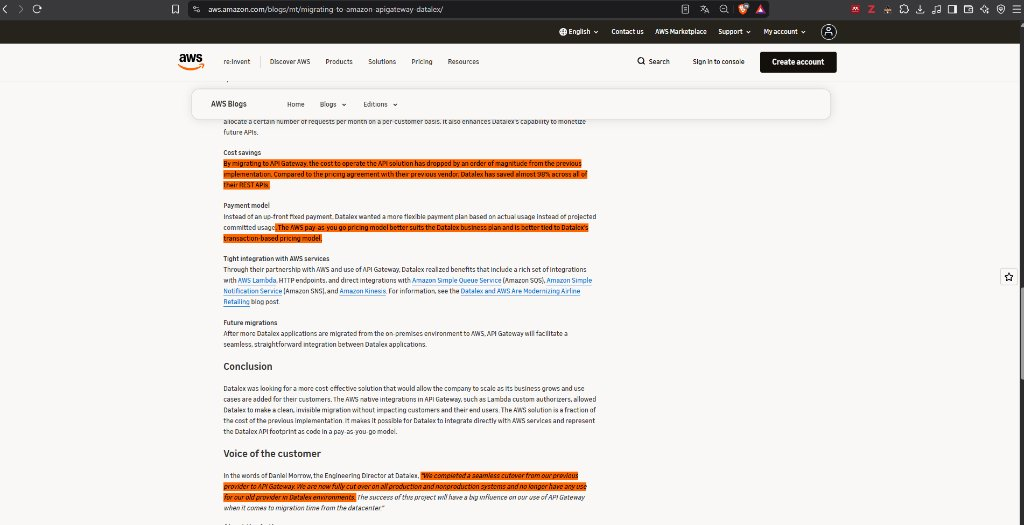
\includegraphics[width=0.92\linewidth]{evidencia_04_resultados_costos_voz.jpg}
  \caption{Evidencia de lectura y subrayado personal de los resultados de negocio (\textit{Cost savings} y \textit{Payment model}) y testimonio de Daniel Morrow (\textit{Voice of the customer}), donde se precisa el alcance del ahorro sobre las API REST y la continuidad del corte. Fuente: Prenty, Morrow y Galan~\cite{prenty2020datalex}.}
  \label{fig:evidencia_04}
\end{figure}

\clearpage

\subsection*{Ejemplo de un sistema conocido de primera mano}
\textit{[Pendiente de redacci\'on propia del estudiante: identificar un sistema real usado o trabajado de primera mano en el que se reconozca el patr\'on API Gateway, diferenci\'andolo t\'ecnicamente de una API REST simple, un proxy inverso o una arquitectura completa de microservicios, y explicando qu\'e funciones centraliza.]}

\subsection*{Declaraci\'on de uso de inteligencia artificial}
Conforme a las normas de integridad acad\'emica del encuadre de la asignatura, la Tabla~\ref{tab:declaracion_ia} estructura el registro del apoyo recibido mediante herramientas de inteligencia artificial, pendiente de revisi\'on y confirmaci\'on final del estudiante.

\begin{table}[htbp]
  \centering
  \small
  \caption{Registro preliminar de apoyo con herramientas de inteligencia artificial (pendiente de confirmaci\'on final del estudiante).}
  \label{tab:declaracion_ia}
  \begin{tabular}{@{}p{2.0cm}p{2.3cm}p{2.8cm}p{3.8cm}p{3.1cm}@{}}
    \toprule
    \textbf{Herramienta} & \textbf{Versi\'on / modelo} & \textbf{Finalidad del uso} & \textbf{Actividades de apoyo realizadas} & \textbf{M\'etodo de verificaci\'on} \\
    \midrule
    ChatGPT & [Confirmar versi\'on real] & Apoyo en investigaci\'on inicial y orientaci\'on metodol\'ogica. & [Confirmar actividades espec\'ificas realizadas con ChatGPT.] & [Confirmar c\'omo se contrast\'o cada resultado.] \\
    \addlinespace
    Antigravity & [Confirmar versi\'on / modelo real] & Apoyo en organizaci\'on documental, b\'usqueda bibliogr\'afica y estructura \LaTeX. & Preparaci\'on de estructura del repositorio, gu\'ia t\'ecnica, plantilla \LaTeX{} y contraste inicial de fuentes y DOI. & Lectura directa de la fuente AWS, apertura y revisi\'on de PDFs y DOI oficiales, subrayado personal y ajuste manual de \texttt{referencias.bib}. \\
    \bottomrule
  \end{tabular}
\end{table}

\noindent\textbf{Responsabilidad del estudiante:} \textit{[Pendiente de confirmaci\'on final: declarar expresamente que el an\'alisis t\'ecnico, las decisiones de dise\~no aplicadas al PFC, el ejemplo de primera mano y la verificaci\'on de las fuentes y citas son de autor\'ia y responsabilidad exclusiva de Luis Alberto Paca Pilataza.]}

\clearpage

% ------------------------------------------------------------------------------
% Referencias (BibLaTeX + estilo IEEE + backend Biber)
% ------------------------------------------------------------------------------
\printbibliography[title={Referencias}]

\end{document}
